\section{Context Oriented nesC (ConesC)}
To mention: detailed description of ConesC, using Wildlife tracking application.

Programming in ConesC is tightly coupled with environment-dependent behavior of the application and exploits two main concepts: \emph{i)} individual contexts and their transitions and \emph{ii)} context groups. The former represent different environment situations where a system may find itself. Each context maps a separate state of application-level or system-level. As the environment conditions change, a programmer initiates a context transition by \emph{activating} corresponding context. Context group is a set of contexts sharing common characteristics. Thus, whenever a transition between involved contexts occurs it is determined by changes in the same physical quantity.

\begin{figure}[!h]
\centering
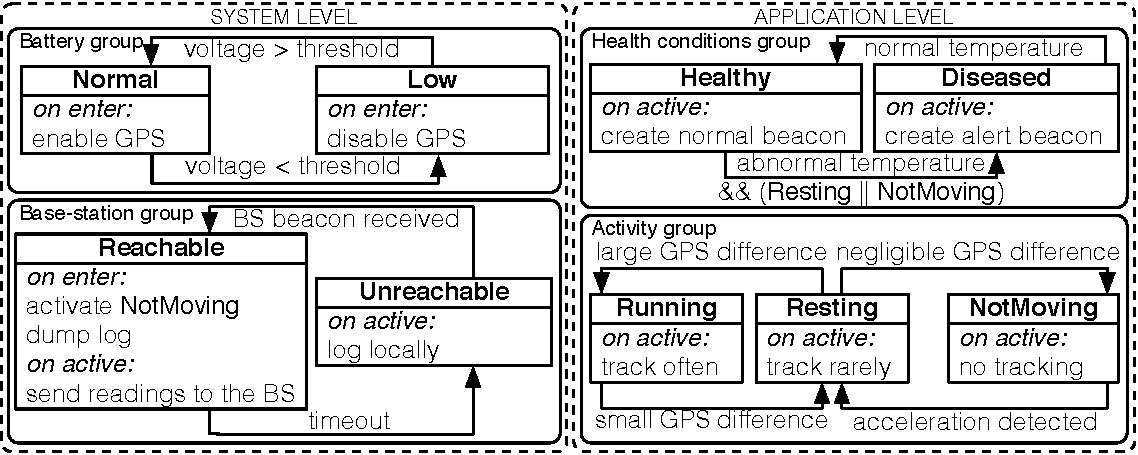
\includegraphics[width=\columnwidth]{pdf/wildlifetracking}
\caption{Diagram}
\label{fig:wtd}
\end{figure}

Diagram on a figure ? displays contextual situations, which may occur during the execution. To reflect this diagram on a language level, ConesC utilizes new types of components, such as \emph{context} and \emph{context configuration}, and a set of new key-words.

\emph{Context} and \emph{context group} types are extensions of \emph{module} and \emph{configuration} correspondingly. However they also can be used as standard nesC components. E.g. one can provide or use interfaces inside instances of these new component types as well as declare them in the same way.  

\emph{Context configuration} component logically represents a context group and is intended to declare layered functions (line ?) as well as included contexts (line ?). Here key-word \emph{layered} means that the behavior of this function depends on activated context. The declaration of contexts follows a key-word \emph{contexts}, but it can be moved in \emph{components} declaration, since the key-word \emph{contexts} was introduced only for convenience and \emph{context} can be declared as a standard component. It is mandatory, however, to declare \emph{default} context, which will be activated at the beginning of the execution, by using key-word \emph{is default}. ConesC also supports a declaration of \emph{error} context for each group by the key-word \emph{is error}. Error context is used to indicate errors occurred during the execution. If error context is not declared, it will be generated automatically.

\begin{Sbox}
\begin{minipage}{\columnwidth}
\begin{csource}
(*@\textbf{context configuration}@*) Location {
(*@\lstnote{layereddef}\textbf{layered}@*) command void report();}
implementation {
(*@\lstnote{contexts}\textbf{contexts}@*) Outdoor,
(*@\lstnote{isdefault}@*) Indoor (*@\textbf{is default}@*);
 components Routing, Logging, 
 LedsC;
 Indoor.Collection -> Routing;
 Outdoor.DataStore -> Logging;
 Error.Leds -> LedsC;}
\end{csource}
\end{minipage}
\end{Sbox}
\begin{figure}
 \TheSbox
 \caption{Context configuration component.}
 \label{fig:ccc}
\end{figure}

\emph{Context} component includes a context-specific implementation of layered function declared in context configuration. Since only one context in a group can be active at a time, a behavioral variation is enabled by this implementation. Programmer may want to add some instructions after context activation such as initialization of variables or enabling/disabling modules (in our example, enable GPS-sensor on entering in \emph{no BS} context). Or it may be necessary to reset component's state before context deactivation. ConesC allows to do this by implementing events \emph{activated()} and \emph{deactivated()} correspondingly, it is not obligatory though. In order to double check if context is really taking place during context transition and avoid false positives, ConesC provides a \emph{check()} command. It as also not mandatory to implement this command, but should it return \emph{FALSE}, an initiated context transition will not occur, a context will not be activated and a system will remain in the previous state. This approach allows one not to think about conditions a transition taking place under, but foresee possible conflicts.

Along with declaration of a new component types, ConesC also allows to specify rules and dependencies for context transitions. In our application for example within Locator group a transition from \emph{not moving} to \emph{resting} is only possible. Since each transition is governed by a separate rule, it is declared in context component as shown on fig ? (line ?). Here key-word \emph{transitions} indicates a list of possible contexts a transition can be performed to. If programmer initiates a transition to a context which is not declared in the rule, an \emph{error} context will be activated.

To map intergroup relations we are introducing a context transition dependencies in our context-oriented language. Withing the \emph{Base Station} group for example a transition from \emph{no BS} to \emph{BS} is only possible if an animal is \emph{running}. Thus, the dependency for this transition is \emph{running} context, which belongs to \emph{Locator} group. Our approach also covers this situation by adding dependencies to the transition declaration as it is shown on a figure ? (line ?). In \emph{transitions} section a context name followed by a key-word \emph{iff} and full name of another context means that the transition will only be executed if the latter context is active. Should the rule with dependency be violated, a transition to an error context will be triggered.

Other type of intergroup relations implies automatic triggering of context transition. Considering \emph{battery} group in our example, we can notice that for further energy saving programmer may want to trigger a transition to \emph{no BS} context withing a \emph{Base Station} group as long as \emph{low} context is active. Our design allows one to do that by declaring a \emph{triggers} section. On a figure ? (line ?) all the declared after this key-word contexts will be activated as soon as a transition to the current context is triggered, all declared rules are satisfied, and implemented \emph{check()} command returns \emph{TRUE}.

to mention: usage